% \documentclass[aspectratio=169]{beamer}
\documentclass[aspectratio=43]{beamer}
\usepackage{tabularx}
\usepackage{booktabs}
\usepackage[utf8]{inputenc}
\usepackage{multirow}
\usepackage{default}
\usepackage{subfigure}
\usetheme{Northwestern}

\title{Using Stochastic Models to Describe and Predict Social Dynamics of Web Users}
\subtitle{Kristina Lerman and Tad Hogg}
\author{Yuanhui Yang}
\institute{Department of Electrical Engineering and Computer Science}
\date{}

\AtBeginSection[]{
  \begin{frame}
    \tableofcontents[ 
        currentsection,
        hideothersubsections, 
        sectionstyle=show/hide, 
        subsectionstyle=show/shaded, 
    ]
  \end{frame}
}

\AtBeginSubsection[]{
  \begin{frame}
    \tableofcontents[ 
        currentsubsection, 
        hideothersubsections, 
        sectionstyle=show/hide, 
        subsectionstyle=show/shaded, 
    ]
  \end{frame}
}

\begin{document}

\maketitle

\begin{frame}{Outline}
  \tableofcontents[pausesections]
  % You might wish to add the option [pausesections]
\end{frame}

\section[Definition]{What is Social Dynamics of Web Users?}
\begin{frame}
% \frametitle{What is Social Dynamics of Web Users?}
\frametitle{Definition and Quantization}
\centering
\begin{minipage}{\textwidth}
\begin{exampleblock}{Definition}
Predicting popularity of content in social media
\end{exampleblock}

\begin{block}{Fact}
If one user interests some social media, he/she will \textbf{\textsl{VOTE}} it
\end{block}

\begin{alertblock}{Quantization}
\begin{itemize}
\item The changing rate of the number of votes at one given time point
\item \begin{equation}
\dfrac{dN_{\mathrm{vote}}\left(t\right)}{dt}
\end{equation}
\end{itemize}
\end{alertblock}
\end{minipage}
\end{frame}

\begin{frame}
\begin{minipage}{\textwidth}
\begin{figure}
\centering
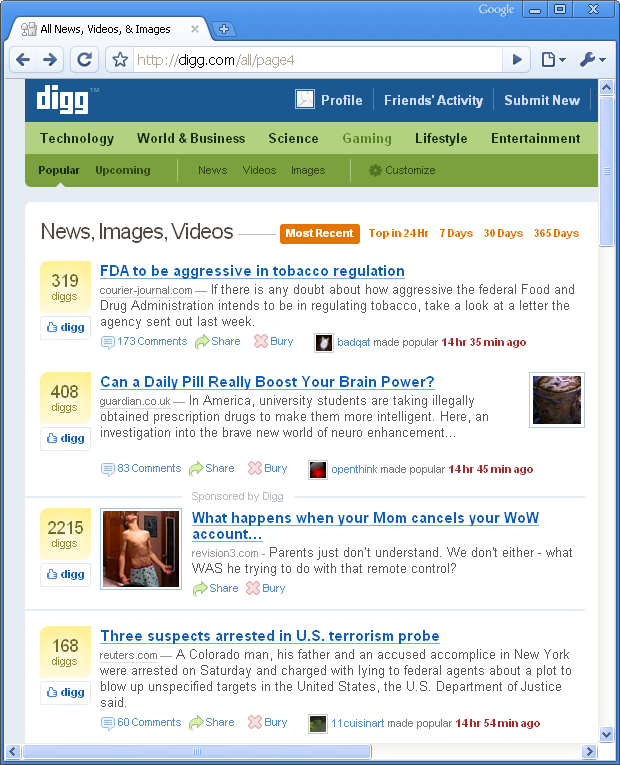
\includegraphics[height=0.8\textheight]{fig01.png}
\caption{Screenshot of the front page of the social news aggregator Digg}
\end{figure}
\end{minipage}
\end{frame}

\section[Value]{Why do they study Social Dynamics of Web Users?}
\begin{frame}
% \frametitle{Why do they study Social Dynamics of Web Users?}
\frametitle{Value}
\centering
\begin{minipage}{\textwidth}
\begin{alertblock}{}
Predicting which newly-submitted items will become popular is critically important for both hosts of social media content and its consumers
\end{alertblock}
\begin{exampleblock}{Hosts Level}
Accurate and timely prediction would enable social media content hosts to maximize revenue through differential pricing for access to content or ad placement
\end{exampleblock}
\begin{block}{Consumers Level}
Prediction would also give consumers an important tool for filtering the ever-growing amount of content
\end{block}
\end{minipage}
\end{frame}

\section[Challenge]{What are the challenges they face?}
\begin{frame}
% \frametitle{What are the challenges they face?}
\frametitle{Challenge}
\centering
\begin{minipage}{\textwidth}
\begin{exampleblock}{Technology Level}
Predicting popularity of content in social media, however, is challenging due to the complex interactions between content quality and how the social media site chooses to highlight content
\end{exampleblock}
\begin{block}{Privacy Level}
Most social media sites also selectively present content that has been highly rated by similar users, whose similarity is indicated implicitly by their behavior or explicitly by links in a social network
\end{block}
\end{minipage}
\end{frame}

\section[Data]{How do they collect their data?}
\begin{frame}
% \frametitle{How do they collect their data?}
\frametitle{Data Collection}
\centering
\begin{minipage}{\textwidth}
\begin{block}{Data Collection}
\begin{itemize}
\item They collected data for the study by scraping Digg's Web pages in May and June 2006
\item structure \{
  \begin{itemize}
  \item the number of votes the stories received
  \item the location of the stories on the upcoming and front pages as a function of time
  \item the names of its early voters
  \end{itemize}
  \}
\end{itemize}
\end{block}
\end{minipage}
\end{frame}

\section[Modeling]{How do they modeling Social Dynamics of Web Users?}
\begin{frame}
\frametitle{Prediction System}
\framesubtitle{State diagram of user behavior for a single story}
\centering
\begin{minipage}{\textwidth}
% \begin{block}{Assumption}
\begin{figure}
\centering
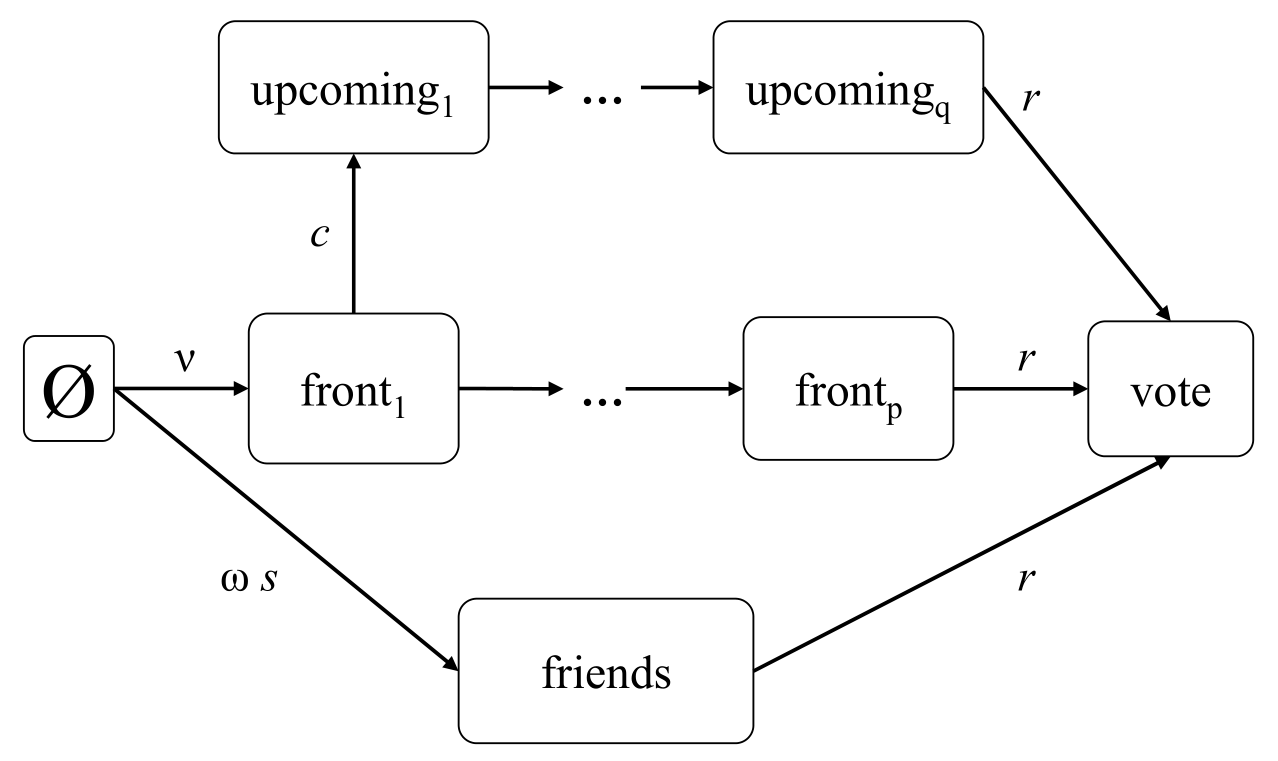
\includegraphics[height=0.7\textheight]{fig02.PNG}
\caption{$vote = function\left(upcomings, fronts, friends\right)$}
\end{figure}
% \end{block}
\end{minipage}
\end{frame}

\begin{frame}
\frametitle{Governing Equation}
% \framesubtitle{State diagram of user behavior for a single story}
\centering
\begin{minipage}{\textwidth}
\begin{block}{Stochastic Master Equation}
\begin{equation}
\begin{array}{lcr}
\dfrac{d\left\langle n_k \right\rangle}{d t} & = & \sum\limits_{j}{\omega_{jk}{\left(\left\langle \vec{n} \right\rangle\right)}{\left\langle{}n_j{}\right\rangle}} - {\left\langle{}n_k{}\right\rangle}\sum\limits_{j}{\omega_{kj}\left(\left\langle{}\vec{n}{}\right\rangle\right)}\\
\dfrac{dN_{\mathrm{vote}}\left(t\right)}{dt} & = & r\left(\nu_f\left(t\right) + \nu_n\left(t\right) + \nu_{\mathrm{friends}}\left(t\right)\right)\\
\end{array}
\end{equation}
\end{block}
\end{minipage}
\end{frame}

\section[Solver]{How do they solve the model?}
\begin{frame}
\frametitle{Solver}
\begin{block}{}
\begin{equation}
\begin{array}{lcr}
f_{\mathrm{page}}{\left(m\right)} & = & \dfrac{1}{2}\left(F_m\left(-\mu\right) - \exp{\left(\frac{2\lambda}{\mu}\right)}F_m\left(\mu\right)\right)\\
F_m\left(x\right) & = & \mathrm{erfc}\left(\alpha_m\dfrac{m - 1 + x}{\mu}\right)\\
p\left(t\right) & = & k_f\left(t-T_{\mathrm{promotion}}\right) + 1\\
q\left(t\right) & = & k_t t + 1\\
\dfrac{ds}{dt} & = & -\omega s + a N_{\mathrm{vote}}^{-b}{\dfrac{dN_{\mathrm{vote}}}{dt}}\\
\end{array}
\end{equation}
\end{block}
\end{frame}

\section[Result]{How is their experimental result?}

\begin{frame}
% \frametitle{How is their experimental result?}
\frametitle{Experimental Result}
\begin{minipage}{\textwidth}
\begin{figure}
\centering
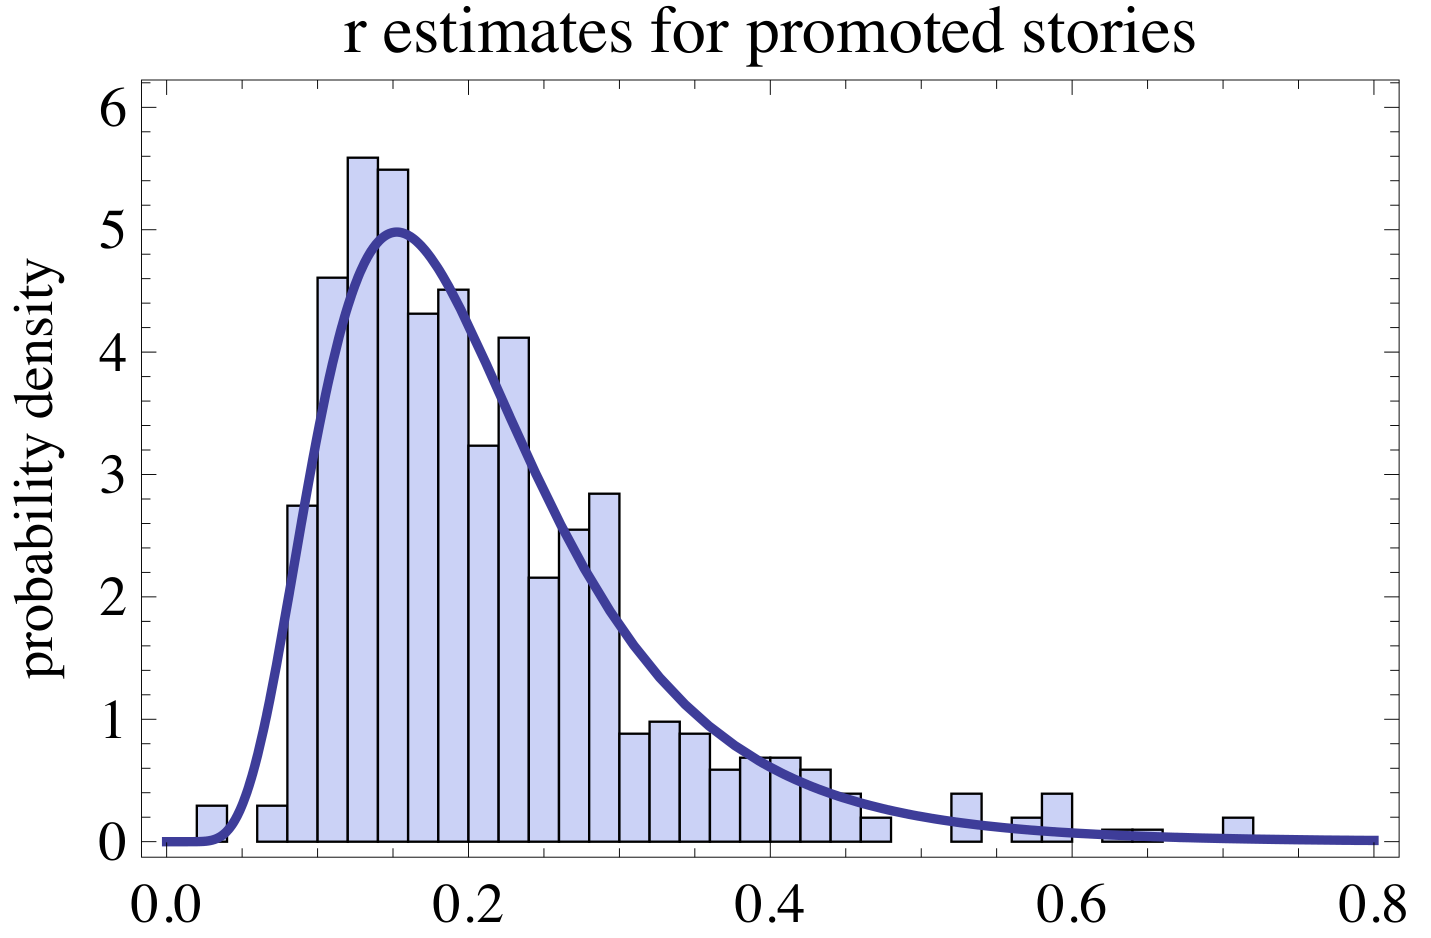
\includegraphics[width=0.8\textwidth]{fig03.PNG}
\caption{Distribution of interestingness (i.e., $r$ values) for the promoted stories in our data set compared with the best fit lognormal distribution.}
\end{figure}
\end{minipage}
\end{frame}

\begin{frame}
% \frametitle{How is their experimental result?}
\frametitle{Experimental Result}
\begin{minipage}{\textwidth}
\begin{figure}
\centering
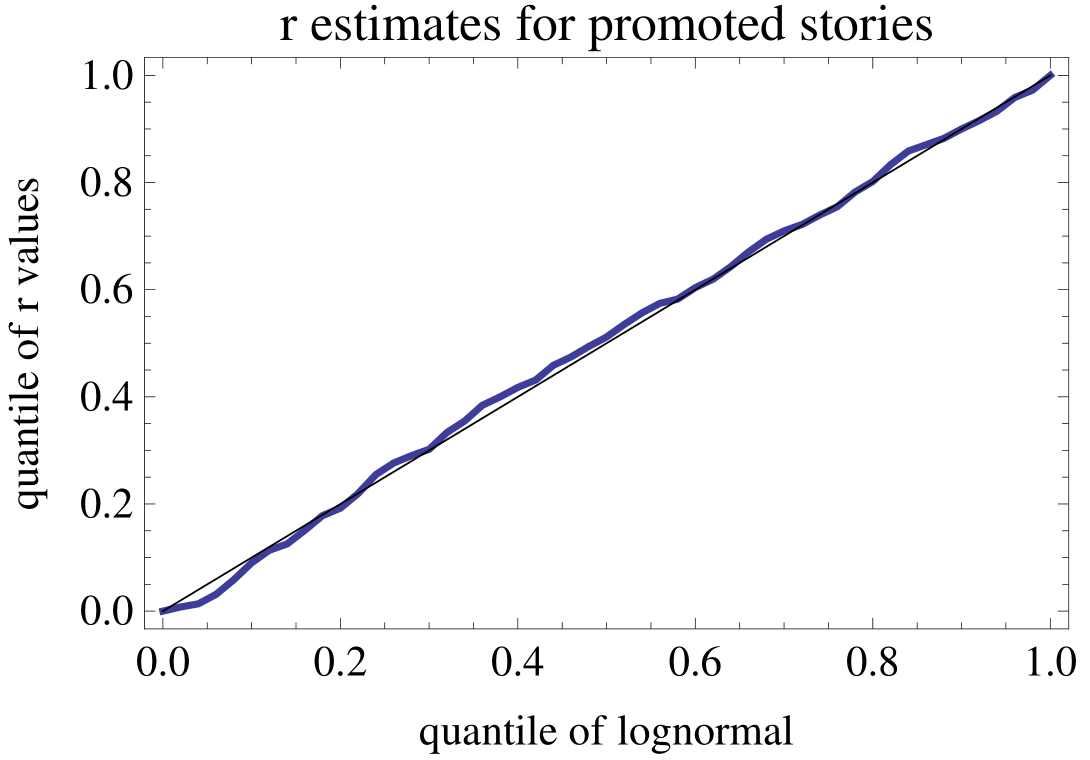
\includegraphics[width=0.8\textwidth]{fig04.PNG}
\caption{Quantile-quantile plot comparing observed distribution of r values with the lognormal distribution fit (thick curve)}
\end{figure}
\end{minipage}
\end{frame}

\section[Modify]{How do they modify this model?}
\begin{frame}
\frametitle{Modification}
\begin{minipage}{\textwidth}
\begin{exampleblock}{}
To investigate differences among voters with respect to the friends network, we extend the previous stochastic model to distinguish votes from fans and non-fans. The model considers the joint behavior of users and the location of the story on
the web site.
\end{exampleblock}
\end{minipage}
\end{frame}
\begin{frame}
\frametitle{A Model of Social Voting with Niche Interests}
\framesubtitle{System Architecture}
\centering
\begin{minipage}{\textwidth}
\begin{figure}
\centering
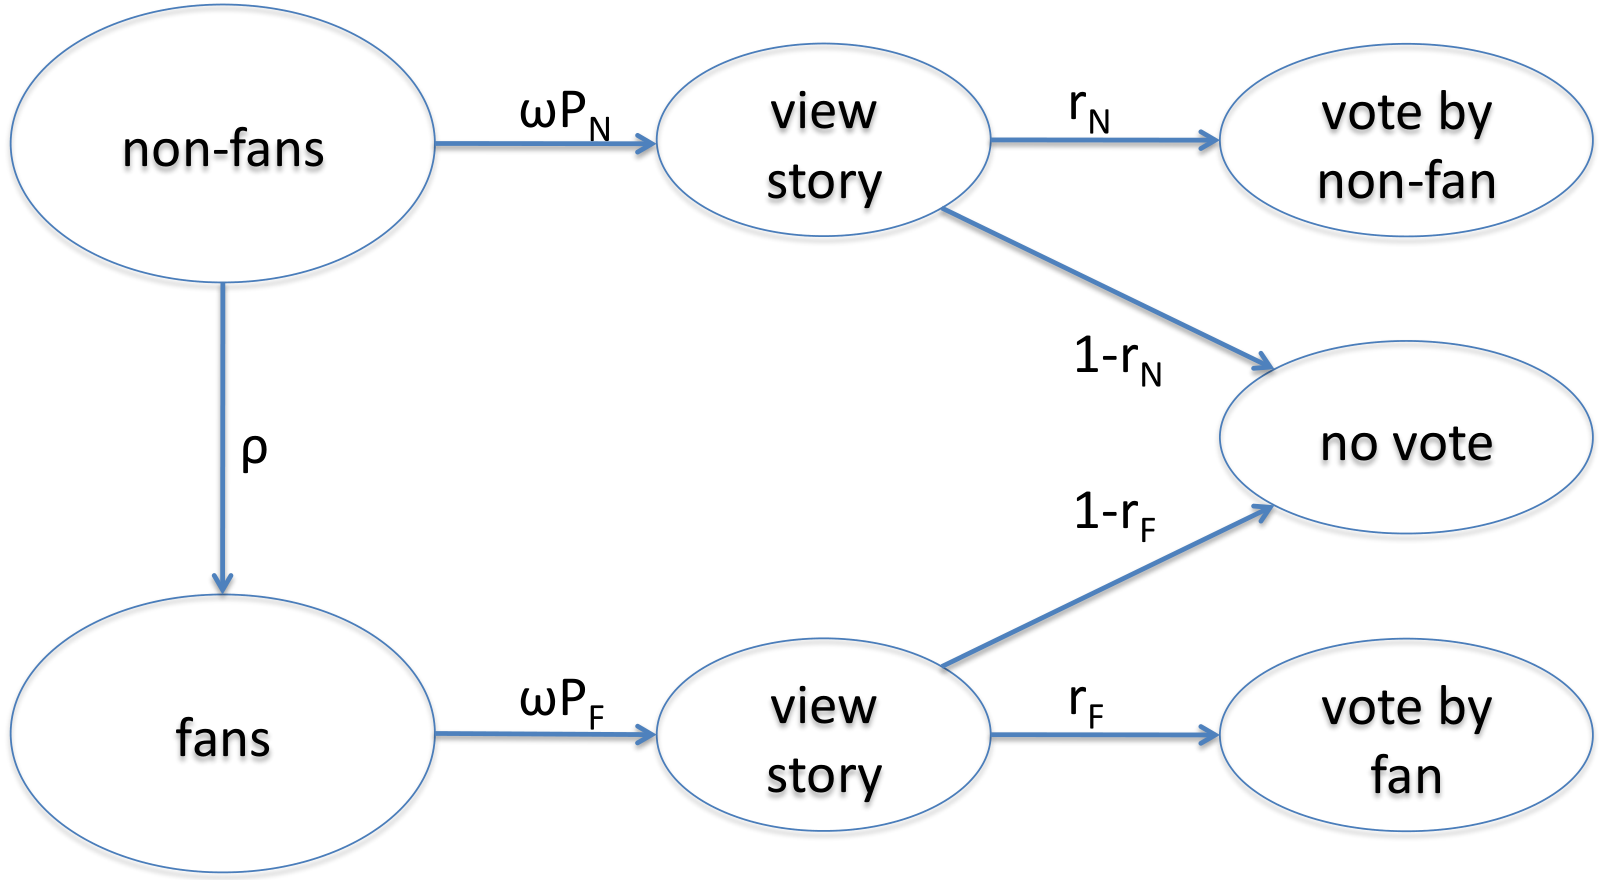
\includegraphics[width=0.8\textwidth]{fig05.png}
\caption{State diagram for a user. The submitter provides a story's first vote.}
\end{figure}
\end{minipage}
\end{frame}

\begin{frame}
\frametitle{A Model of Social Voting with Niche Interests}
\framesubtitle{System Architecture}
\centering
\begin{minipage}{\textwidth}
\begin{figure}
\centering
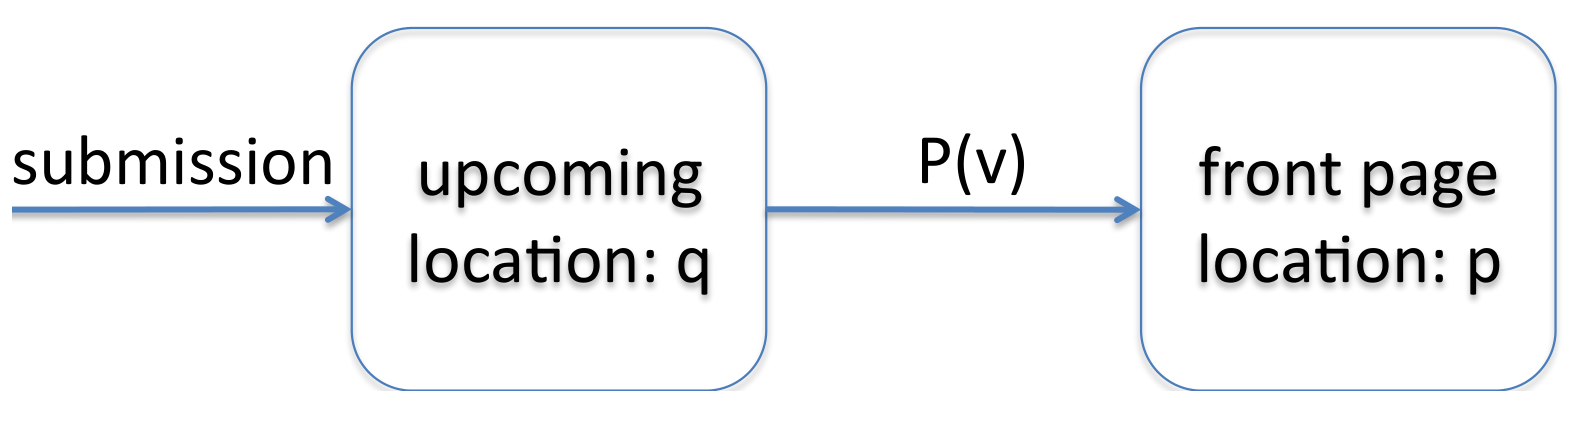
\includegraphics[width=0.8\textwidth]{fig12.PNG}
\caption{State diagram for a story}
\end{figure}
\end{minipage}
\end{frame}

\begin{frame}
\frametitle{Govern Equation}
\begin{minipage}{\textwidth}
\begin{block}{}
  \begin{equation}
	\begin{array}{lcr}
    \dfrac{dv_F}{dt} & = & \omega{}r_F{}P_F{}F\\
    \dfrac{dv_N}{dt} & = & \omega{}r_N{}P_N{}N\\
    \dfrac{dF}{dt} & = & -\omega{}r_F{}P_F{}F + \rho N \dfrac{dv}{dt}\\
    \dfrac{dB}{dt} & = & -\omega{}r_N{}P_N{}N - \rho N \dfrac{dv}{dt}\\
    \end{array}
  \end{equation}
\end{block}
\end{minipage}
\end{frame}

\begin{frame}
\frametitle{Parameter Estimation}
\begin{minipage}{\textwidth}
\begin{figure}
\centering
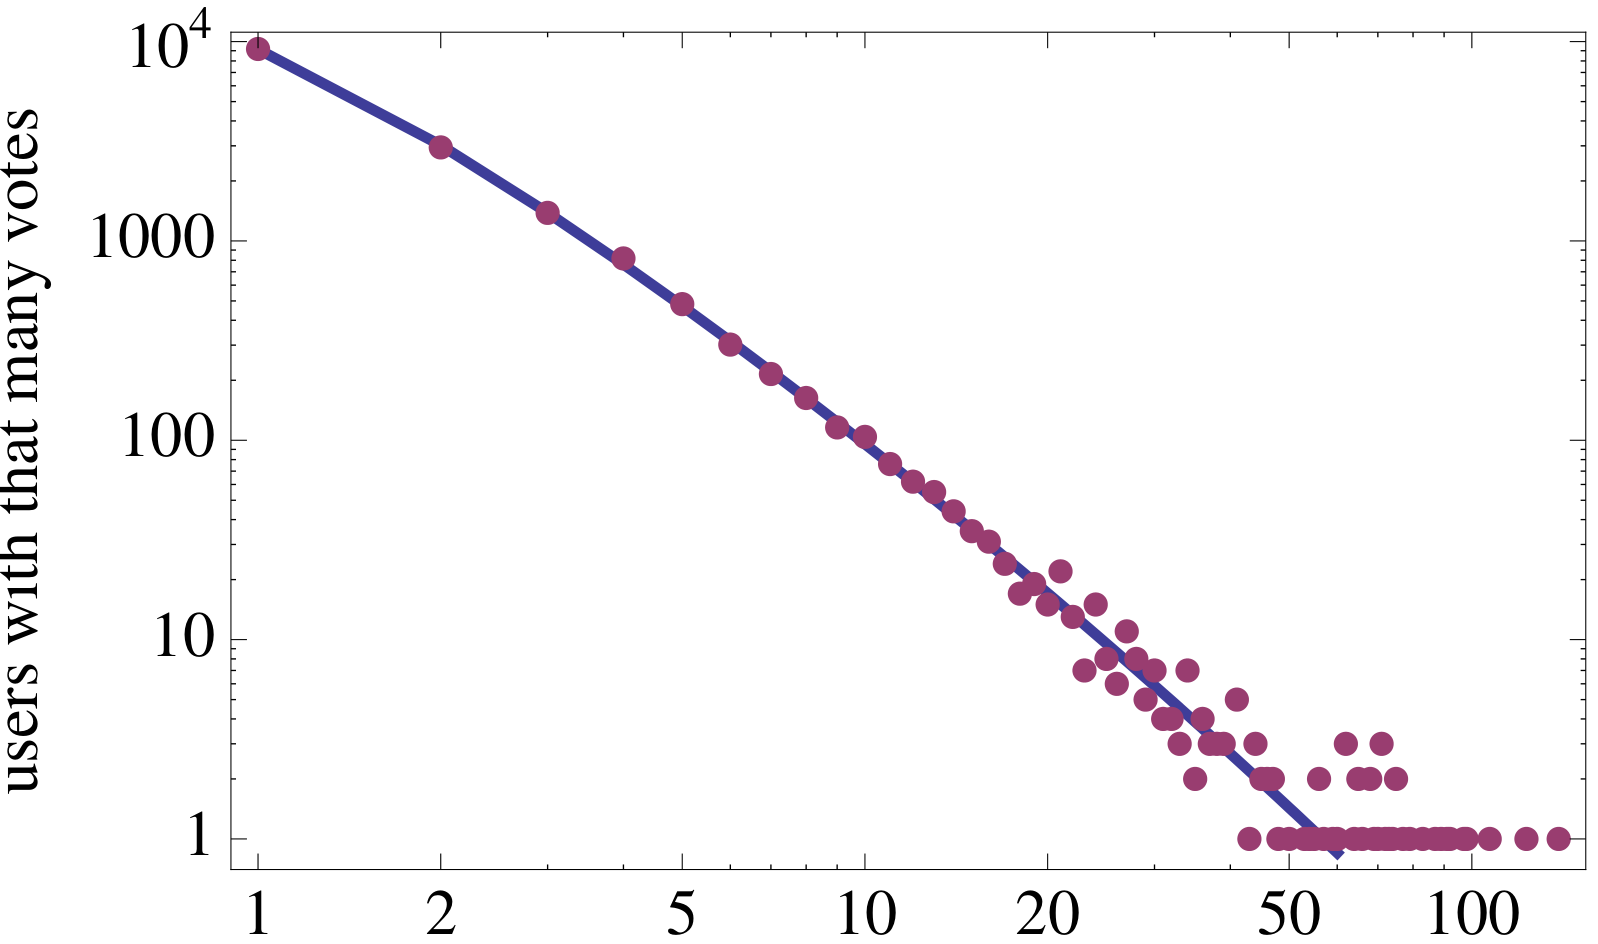
\includegraphics[height=0.7\textheight]{fig06.PNG}
\caption{User activity distribution on logarithmic scales. The curve
shows the fit to the model described in the text.}
\end{figure}
\end{minipage}
\end{frame}

\begin{frame}
\centering
\frametitle{Parameter Estimation}
\begin{minipage}{\textwidth}
\begin{figure}
\centering
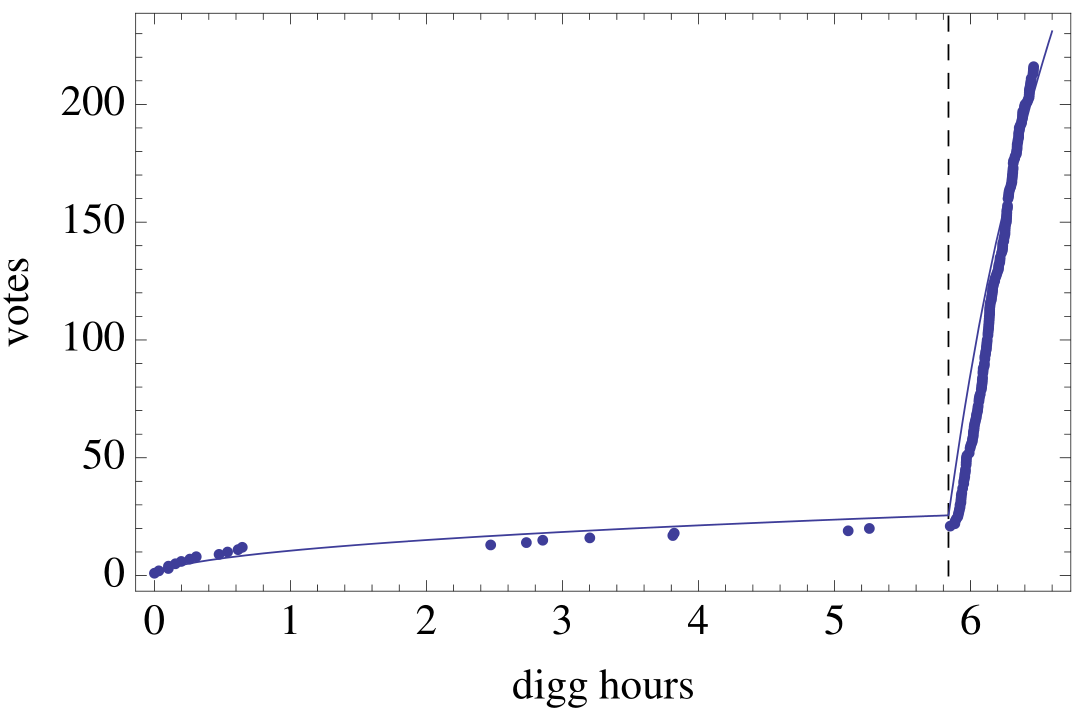
\includegraphics[height=0.7\textheight]{fig07.PNG}
\caption{Voting behavior: the number of votes vs. time, measured in Digg hours, for a promoted story in June 2006.}
\end{figure}
\end{minipage}
\end{frame}

\begin{frame}
\frametitle{Experimental Result}
\centering
\begin{minipage}{\textwidth}
\begin{figure}
\centering
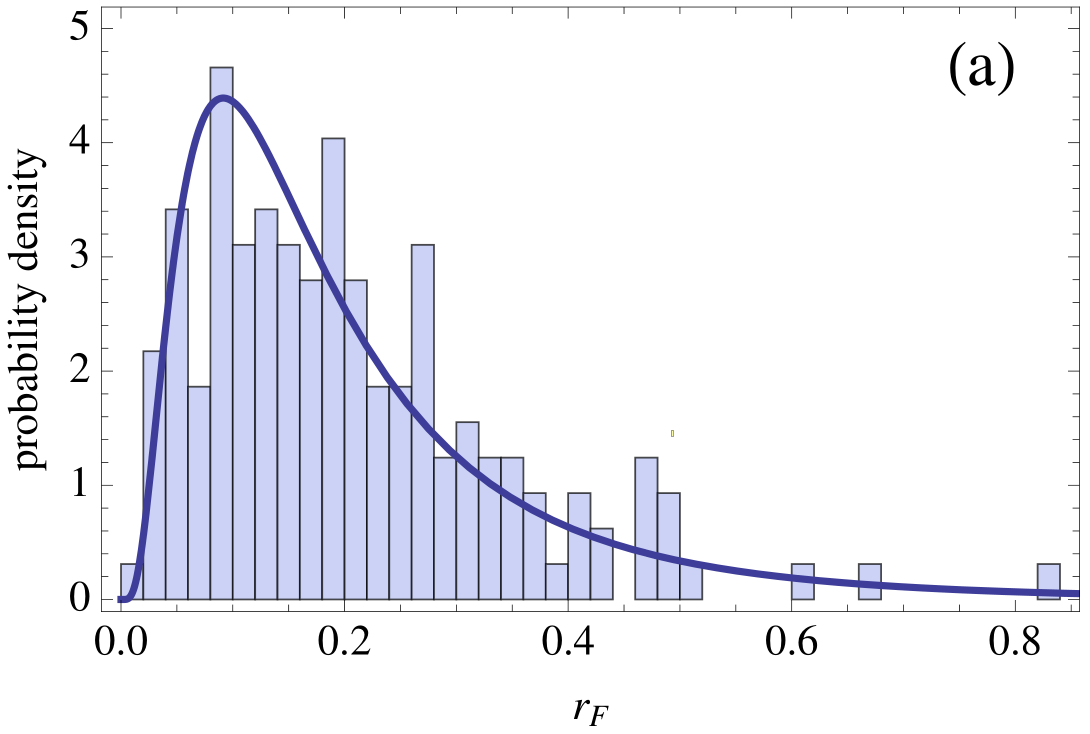
\includegraphics[width=0.8\textwidth]{fig08.PNG}
\caption{Distribution of interestingness for (a) fans}
\end{figure}
\end{minipage}
\end{frame}

\begin{frame}
\frametitle{Experimental Result}
\centering
\begin{minipage}{\textwidth}
\begin{figure}
\centering
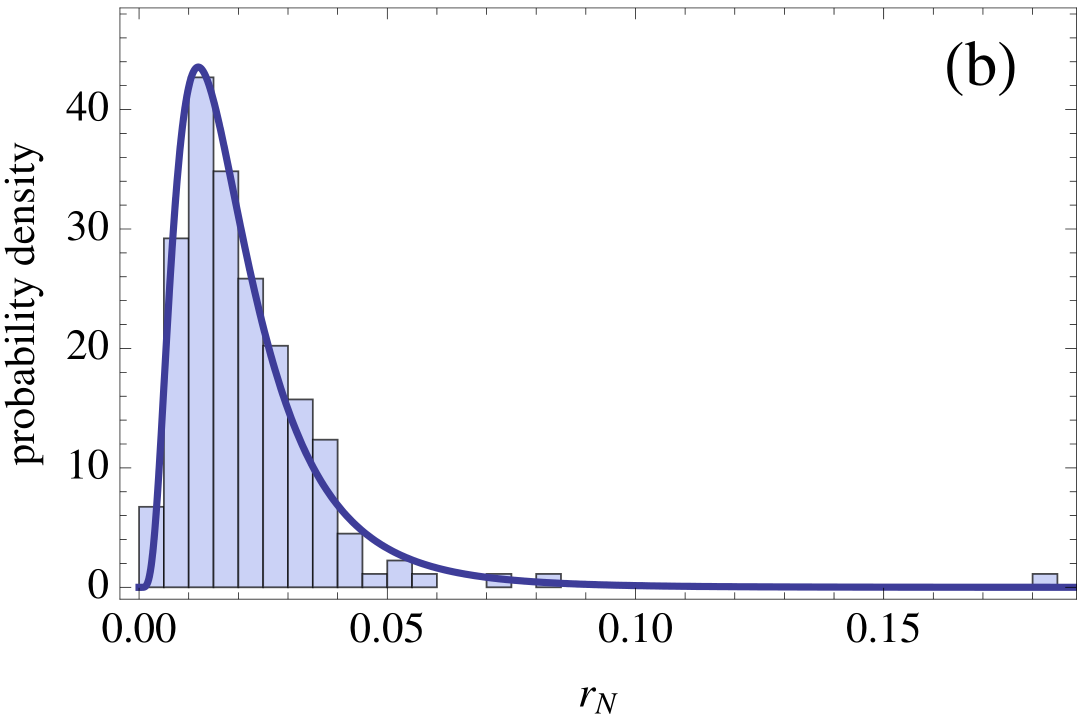
\includegraphics[width=0.8\textwidth]{fig09.PNG}
\caption{Distribution of interestingness for (b) non-fans}
\end{figure}
\end{minipage}
\end{frame}

\begin{frame}
\frametitle{Experimental Result}
\centering
\begin{minipage}{\textwidth}
\begin{figure}
\centering
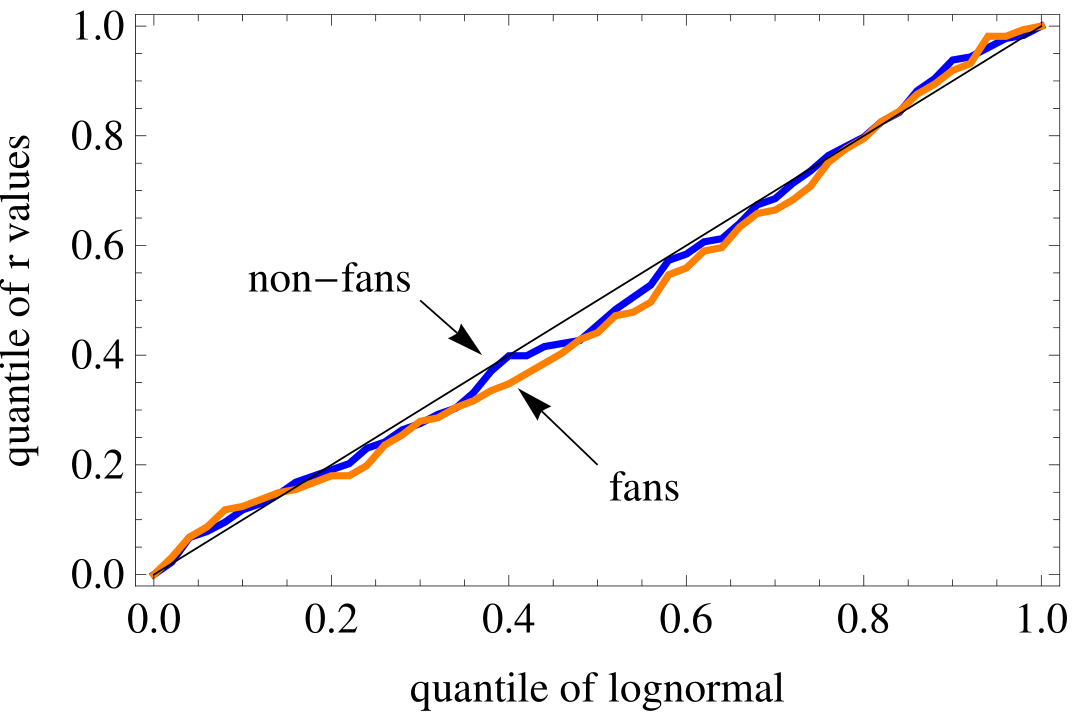
\includegraphics[width=0.8\textwidth]{fig10.PNG}
\caption{ Quantile-quantile plot comparing the observed distribution for $r_F$ (fans) and $r_N$ (non-fans) with the corresponding lognormal distribution fits (thick curves).}
\end{figure}
\end{minipage}
\end{frame}

\begin{frame}
\frametitle{Model-Based Prediction}
\centering
\begin{minipage}{\textwidth}
\begin{figure}
\centering
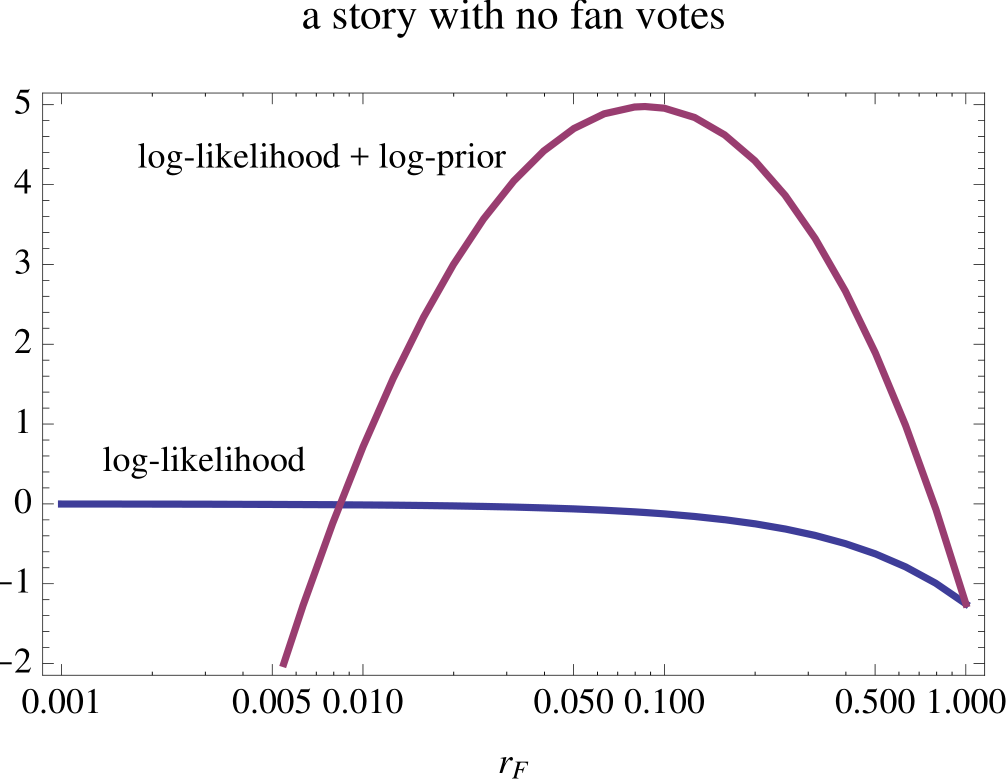
\includegraphics[width=0.7\textwidth]{fig13.PNG}
\caption{Comparisonoflog-likelihood(i.e., logP(r|votes)) and log-likelihood plus $log\left(P prior \left(r\right)\right)$ for estimating $r_F$ for a story with no fan votes.}
\end{figure}
\end{minipage}
\end{frame}

\section[Conclusion]{Conclusion}
\begin{frame}
\frametitle{Conclusion}
% \framesubtitle{Experimental Result}
\centering
\begin{minipage}{\textwidth}
Their solution can partially address this prediction challenge by quantitatively characterizing evolution of popularity.
\end{minipage}
\end{frame}

\begin{frame}
%\frametitle{A first slide}

\begin{center}
\Huge Thank you
\end{center}

\end{frame}
\end{document}
